\fancyhead[L]{\textsf{\textbf{62}}\quad \textsf{CHƯƠNG 1}\quad \textsf{Hàm số và Mô hình}}
\fancyhead[R]{}
\noindent
\begin{minipage}[t]{0.26	extwidth}
    \vspace*{9.8cm}
    \noindent
    \tikz[baseline=-0.6ex]{\draw[stewartred, line width=1.1pt] (0,0) circle (5.5pt); \draw[stewartred, line width=1.1pt] (-3.89pt, 3.89pt) -- (3.89pt, -3.89pt);}\;
    {\small\color{stewartcyan}$\sin^{-1}x \neq \dfrac{1}{\sin x}$}

    \vspace{2.1cm}
    \begin{center}
        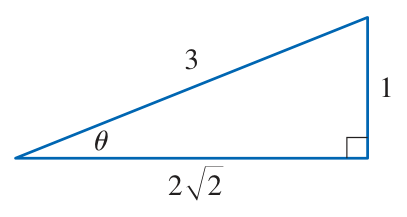
\includegraphics[width=0.92\linewidth]{images/p0097_fig3.png}\\[1.5mm]
        {\small\textbf{\textsf{HÌNH 19}}}
    \end{center}

    \vspace{1.0cm}
    \begin{center}
        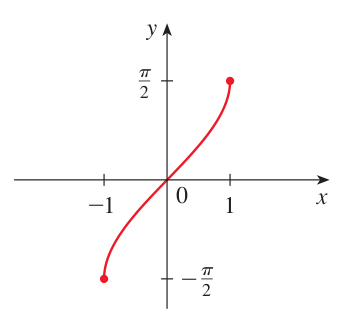
\includegraphics[width=0.88\linewidth]{images/p0097_fig4.png}\\[1.5mm]
        {\small\textbf{\textsf{HÌNH 20}}\\[1mm]
        $y = \sin^{-1} x = \arcsin x$}
    \end{center}
\end{minipage}%
\hfill
\begin{minipage}[t]{0.71	extwidth}
    Từ Hình 17, bạn có thể thấy hàm số sin $y = \sin x$ không phải là hàm một-đối-một (dùng Kiểm tra đường nằm ngang). Tuy nhiên, nếu ta thu hẹp miền xác định vào đoạn $[-\pi/2, \pi/2]$, thì hàm số \textit{là} một-đối-một và nhận mọi giá trị trong tập giá trị của $y = \sin x$ (xem Hình 18). Hàm số ngược của hàm sin thu hẹp $f$ này tồn tại và được ký hiệu là $\sin^{-1}$ hoặc $\arcsin$. Nó được gọi là \textbf{hàm số sin ngược} hay \textbf{hàm arcsin}.

    \vspace{0.28cm}
    \noindent
    \begin{minipage}[t]{0.58\linewidth}
        \centering
        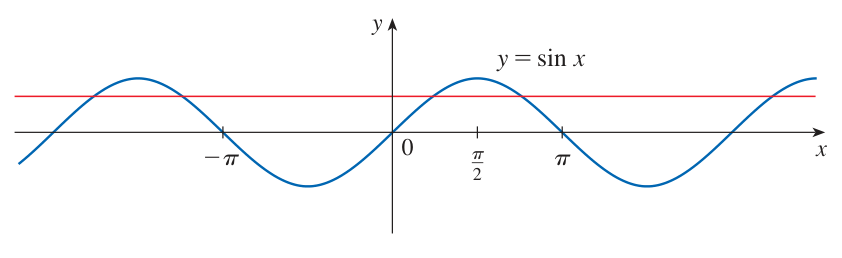
\includegraphics[height=2.35cm, keepaspectratio]{images/p0097_fig1.png}\\[2mm]
        {\small\textbf{\textsf{HÌNH 17}}}
    \end{minipage}\hfill
    \begin{minipage}[t]{0.38\linewidth}
        \centering
        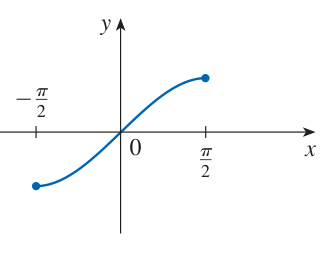
\includegraphics[height=2.35cm, keepaspectratio]{images/p0097_fig2.png}\\[2mm]
        {\small\textbf{\textsf{HÌNH 18}}\\[1mm]
        $y = \sin x,\; -\frac{\pi}{2} \leqslant x \leqslant \frac{\pi}{2}$}
    \end{minipage}

    \vspace{0.25cm}
    Vì định nghĩa của hàm ngược phát biểu rằng
    \[
    f^{-1}(x) = y \iff f(y) = x
    \]
    nên ta có

    \vspace{-0.2cm}
    \begin{center}
        \begin{tcolorbox}[colframe=stewartred, colback=white, sharp corners, boxrule=0.8pt, width=0.92\linewidth, halign=center, top=5pt, bottom=5pt]
            $\sin^{-1}x = y \iff \sin y = x \quad \text{và} \quad -\dfrac{\pi}{2} \leqslant y \leqslant \dfrac{\pi}{2}$
        \end{tcolorbox}
    \end{center}

    \vspace{0.08cm}
    Do đó, nếu $-1 \leqslant x \leqslant 1$, thì $\sin^{-1}x$ là số nằm giữa $-\pi/2$ và $\pi/2$ có sin bằng $x$.

    \vspace{0.25cm}
    \noindent
    \textbf{\textsf{\color{stewartcyan}VÍ DỤ 13}}\quad Tính (a) $\sin^{-1}\left(\frac{1}{2}\right)$ và (b) $\tan\left(\arcsin\frac{1}{3}\right)$.

    \vspace{0.12cm}
    \noindent
    \textbf{\textsf{\color{stewartcyan}LỜI GIẢI}}

    \noindent
    (a) Ta có
    \[
    \sin^{-1}\left(\frac{1}{2}\right) = \frac{\pi}{6}
    \]
    bởi vì $\sin(\pi/6) = \frac{1}{2}$ và $\pi/6$ nằm giữa $-\pi/2$ và $\pi/2$.

    \vspace{0.12cm}
    \noindent
    (b) Đặt $\theta = \arcsin\frac{1}{3}$, suy ra $\sin\theta = \frac{1}{3}$. Khi đó ta có thể vẽ một tam giác vuông có góc $\theta$ như trong Hình 19 và suy ra từ Định lý Pythagoras rằng cạnh thứ ba có độ dài bằng $\sqrt{9 - 1} = 2\sqrt{2}$. Điều này cho phép ta đọc được từ tam giác rằng
    \[
    \tan\left(\arcsin\frac{1}{3}\right) = \tan\theta = \frac{1}{2\sqrt{2}} \tag*{{\color{stewartcyan}$\blacksquare$}}
    \]

    Các phương trình triệt tiêu đối với hàm ngược trong trường hợp này trở thành

    \vspace{-0.2cm}
    \begin{center}
        \begin{tcolorbox}[colframe=stewartred, colback=white, sharp corners, boxrule=0.8pt, width=0.92\linewidth, halign=center, top=6pt, bottom=6pt]
            \begin{align*}
                \sin^{-1}(\sin x) &= x \quad \text{với} \quad -\frac{\pi}{2} \leqslant x \leqslant \frac{\pi}{2} \\[2mm]
                \sin(\sin^{-1}x) &= x \quad \text{với} \quad -1 \leqslant x \leqslant 1
            \end{align*}
        \end{tcolorbox}
    \end{center}

    \vspace{0.08cm}
    Hàm số sin ngược, $\sin^{-1}$, có tập xác định là $[-1, 1]$ và tập giá trị là $[-\pi/2, \pi/2]$, và đồ thị của nó, được vẽ trong Hình 20, nhận được từ đồ thị của hàm số sin thu hẹp (Hình 18) bằng phép lấy đối xứng qua đường thẳng $y = x$.
\end{minipage}